% small.tex
\documentclass{beamer}
%include polycode.fmt
\usepackage{xcolor}
\usepackage{media9}
\usepackage{tikz}
\usetikzlibrary{patterns}
\usepackage{pgfplots}
\usepackage[normalem]{ulem}
\usepackage{color, colortbl}
\usepackage{tikz}
\usetikzlibrary{arrows,%
                shapes,positioning}
\usetikzlibrary{trees}
\usetikzlibrary{shapes}
\definecolor{green}{rgb}{0,1,0}
\definecolor{navyblue}{rgb}{0.2,0.2,0.7}
\usetheme{Antibes}
\useoutertheme[subsection=false]{miniframes}
\usenavigationsymbolstemplate{}
\newsavebox\MBox
\newcommand\Cline[2][red]{{\sbox\MBox{$#2$}%
  \rlap{\usebox\MBox}\color{#1}\rule[-1.2\dp\MBox]{\wd\MBox}{0.5pt}}}
  
\title{Monadic Functional Reactive Programming}
\author{Atze van der Ploeg}
\institute{
Centrum Wiskunde \& Informatica, Amsterdam, The Netherlands}

\newcommand{\dfcode}[1]{\begin{flalign*}\vspace{-0.35cm}#1\vspace{-0.35cm}\end{flalign*}}
\newcommand{\mul}{\!\times\!}
% \date{\today}

\newcommand{\frameofframes}{/}
\newcommand{\setframeofframes}[1]{\renewcommand{\frameofframes}{#1}}
\makeatletter
\setbeamertemplate{footline}
  {%
   
\hfill%
      {\usebeamerfont{frame number}\usebeamercolor[fg]{frame number}\insertframenumber~\frameofframes~\inserttotalframenumber}
  }
\makeatother

\begin{document}

% \AtBeginSection[]
% {
%    \begin{frame}
%        \frametitle{Outline}
%        \tableofcontents[currentsection]
%    \end{frame}
% }


%--- the titlepage frame -------------------------%

\begin{frame}[plain]
\begin{center}
  \scalebox{12}{$\bind$}
\end{center}
\vspace{-0.5cm}
  \titlepage
\end{frame}

\section{Intro}

%format Reactg = "\mathit{React}_{\!\mkern+0.4mu\mathit{g}}"
%format <*> = "\ap"
%format <<< = "<\!\!\!<\!\!\!<"
%format >>> = ">\!\!\!>\!\!\!>"
%format *** = "*\!\!*\!\!*"
%format -< = "\:-\!\!\!<"
%format Sigg   = "\mathit{Sig}_{\!\mathit{g}}"
%format <&&> = "<\!\!\!\$\!\$\!\!\!>"
%format >>> = ">\!\!\!>\!\!\!>"
%format *** = "*\!\!*\!\!*"
%format &&& = "\:\&\!\!\&\!\!\&\:"
%format ~= = "\approx"


\newcommand{\inlineitem}{%
{\color{navyblue} \leavevmode\usebeamertemplate{itemize item} }
}

\begin{frame}{Transformational vs. Reactive}
\begin{block}{Transformational program}
Transforms input into output.\\

Examples:
\begin{itemize}
\item Traditional compiler
\item Long-running scientific computation
\end{itemize}
\end{block}

\begin{block}{Reactive program}
Engages in a dialogue with its environment, responding to events.\\

Examples:
\begin{itemize}
\item IDE
\item Spreadsheet
\item Anything with a GUI
\end{itemize}
\end{block}
\end{frame}


\begin{frame}{Why Functional Reactive Programming?}
\begin{block}{Reactive programming means...}
Dealing with external events which may occur in \alert{in any order}.\\
\vspace{0.2cm}
Traditional approaches:\\
\begin{tabular}{l l l}
\inlineitem & Concurrency &\only<2->{$\rightarrow$ non-determinism}\\
\inlineitem & Blocking I/O multiplexing &\only<2->{$\rightarrow$ non-composable}\\
\inlineitem & Callbacks (observer pattern) & \only<2->{$\rightarrow$ inversion of control} \\
\end{tabular}
\end{block}
\pause
\pause

\begin{block}{Functional reactive programming}
is \alert{deterministic}, \alert{composable} and \alert{without inversion of control}.
\end{block}


\end{frame}
    
\begin{frame}{Functional Reactive Programming basics}

\begin{block}{Behaviors}
A \alert{behavior} is a value that changes over time.
Example: The mouse position.
\end{block}

\begin{block}{Events}
An \alert{event} (source) is a behavior that occasionally holds a value.\\
I.e. |Event a ~= Behavior (Maybe a)|\\
Example: Mouse clicks.
\end{block}
\end{frame}



\begin{frame}<1>[label=overview]{Talk overview}
\begin{enumerate}
\item A monadic programmer interface for FRP
\begin{itemize}
\item Problem
\item Solution
\end{itemize}
\item \only<1>{Evaluation mechanism} \only<2>{\alert{Evaluation mechanism}}
\begin{itemize}
\item Problem
\item Solution
\end{itemize}
\end{enumerate}
\end{frame}




\section{Programmer interface}
\newlength{\tmathindenta}
\setlength{\tmathindenta}{\mathindent}
\setlength{\mathindent}{0.15cm}

\begin{frame}{Traditional way of composing behavioral phases}
\begin{code}
switcher :: Behavior a -> Event (Behavior a) -> Behavior a
\end{code}
\pause
\vspace{-0.5cm}
\begin{block}{Example}
\vspace{-0.4cm}
\begin{center}
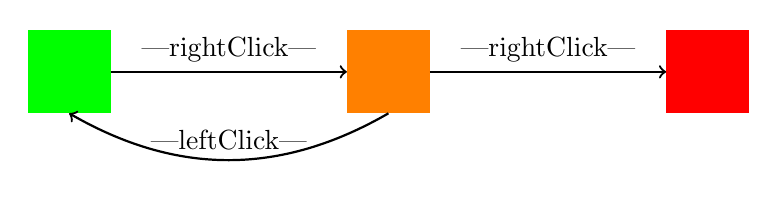
\begin{tikzpicture}[node distance=3cm]
\tikzset{VertexStyle/.style = {shape          = rectangle,
                                 inner sep      = 2pt,
                                 outer sep      = 0pt,
                                 minimum size   = 30 pt}}
     \node[VertexStyle,fill=green](G){};
     \node[VertexStyle,fill=orange,right=of G](OR){};
     \node[VertexStyle,fill=red,right=of OR](R){};   
     %\draw[EdgeStyle](B) to node[LabelStyle]{1} (D) ;
     %\tikzset{EdgeStyle/.append style = {bend left}}
     \draw[thick,->](G) to node[above]{|rightClick|} (OR);
     \draw[thick,->](OR) to node[above]{|rightClick|} (R);
     \draw[thick,->,bend left](OR.south) to node[above]{|leftClick|} (G.south);

  \end{tikzpicture}
\end{center}
\vspace{-0.8cm}
\pause

\begin{code}
traffic :: Behavior Color
traffic = 
  pure green  `switcher`  (rightClick                    <&&> \_ -> 
  pure orange `switcher`  (tagBool leftClick rightClick  <&&> \r ->
  if r then traffic else pure red))
(<&&>) = flip fmap
tagBool :: Event a -> Event b -> Event Bool
\end{code}
\setlength{\mathindent}{\tmathindenta}
\vspace{-0.8cm}
\end{block}
\pause
Question: \alert{Why can't we use |>>=|?}
\end{frame}
\begin{frame}{Monadic FRP definitions}
Answer: We cannot use |>>=| because behaviors cannot \alert{end}.
\vspace{0.3cm}
\begin{block}{Signal computation}
A behavior that may end. \\
|Sigg| has two type arguments:
\begin{itemize}
\item The type of the values of the behavior.
\item The type of the value that it returns.
\end{itemize}
\vspace{-0.5cm}
\begin{code}
instance Monad (Sigg b) where ...
\end{code}
\vspace{-0.8cm}
\end{block}
\pause
\begin{block}{Reactive computation}
A signal computation that gives no information, except when it ends.
\end{block}
\vspace{-0.25cm}


\begin{code}
type Behaviour  a  = Sigg a Void
type Reactg     a  = Sigg () a
type Event      a  = Sigg (Maybe a) Void
\end{code}

\end{frame}


\begin{frame}{Monadic way of composing behavioral phases}

\begin{block}{Example}
\vspace{-0.4cm}
\begin{center}
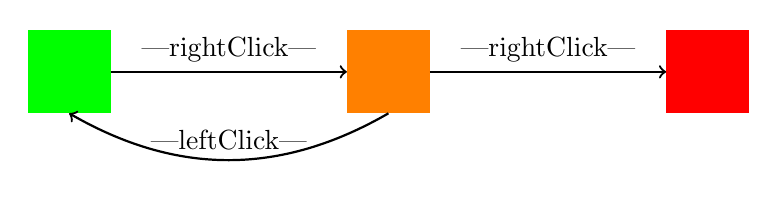
\begin{tikzpicture}[node distance=3cm]
\tikzset{VertexStyle/.style = {shape          = rectangle,
                                 inner sep      = 2pt,
                                 outer sep      = 0pt,
                                 minimum size   = 30 pt}}
     \node[VertexStyle,fill=green](G){};
     \node[VertexStyle,fill=orange,right=of G](OR){};
     \node[VertexStyle,fill=red,right=of OR](R){};   
     %\draw[EdgeStyle](B) to node[LabelStyle]{1} (D) ;
     %\tikzset{EdgeStyle/.append style = {bend left}}
     \draw[thick,->](G) to node[above]{|rightClick|} (OR);
     \draw[thick,->](OR) to node[above]{|rightClick|} (R);
     \draw[thick,->,bend left](OR.south) to node[above]{|leftClick|} (G.south);

  \end{tikzpicture}
\end{center}
\vspace{-0.6cm}


\begin{code}
traffic :: Sigg Color Void
traffic = 
  do  always green `until'` rightClick
      l <- always orange `until'` (rightClick `before` leftClick)
      if l then traffic else always red
\end{code}
\begin{code}
always  :: a -> Sigg a Void
until'  :: Sigg a Void -> Reactg b -> Sigg a b
before  :: Reactg x -> Reactg y -> Reactg Bool
\end{code}
\setlength{\mathindent}{\tmathindenta}
\vspace{-0.8cm}
\end{block}
\end{frame}


\section{Evaluation mechanism}
\againframe<2>{overview}


\begin{frame}<1>[label=evalmot]{The problem with existing evaluation mechanisms}
\begin{block}{Other FRP evaluation mechanisms either ...}
\begin{tabular}{l p{0.5\textwidth} || p{0.35\textwidth}}
\inlineitem & Re-evaluate whole expression after each event &$\rightarrow$ Inefficient\\
\inlineitem & Use side-effects to prevent redundant re-evaluations &$\rightarrow$ \only<1>{?}\only<2->{No time-branching}\\
\end{tabular}
\end{block}
\pause
\pause

\begin{block}{Monadic FRP ...}
has the first \emph{purely functional} evaluation mechanism that prevents redundant re-evaluations
\end{block}

\end{frame}

\begin{frame}{Time-branching}
Suppose that drawings in a drawing program are signal computations:
\vspace{-0.5cm}
\begin{center}
\includegraphics[scale=0.3]{drawing.pdf}\\
\end{center}
Time-branching: ``Freeze'' a running signal computation.\\

Example usages:
\begin{itemize}
\item Duplicate drawing in drawing program into two tabs
\item Undo
\item What-if?
\end{itemize}

\pause
\alert{Impossible} with impure evaluation mechanism


\end{frame}
\againframe<2-3>{evalmot}

\begin{frame}{Basic building blocks of Monadic FRP}
Reminder:
\begin{block}{Reactive computation}
A signal computation that gives no information, except when it ends.\\
\begin{code}
type Reactg     a  = Sigg () a
\end{code}
\end{block}

\begin{itemize}
\item Actually: signal computations are defined in terms of reactive computations.
\item All Monadic FRP expression are built using:
  \begin{itemize}
    \item Sequential composition: |>>=|
\item Parallel composition:  |first|
\end{itemize}
\end{itemize}



\end{frame}

\centering
\tikzstyle{bag} = [rectangle,text centered,draw=black,semithick,solid]
\tikzstyle{interpret} = [rectangle, rounded corners,text centered,draw=black,semithick]
 \tikzstyle{every node}=[font=\small]

\begin{frame}{Example evaluation}

\begin{tikzpicture}[grow=down, level distance=60pt]
[-]

\node[bag, name=root] {|first|}
  [sibling distance=4.5cm]
  child {node[bag] {|first|}[sibling distance=2cm]
    child {node[bag] {|mouseMove|}
       edge from parent[<-]
       node[xshift=-15pt,midway,fill=white,color=white,text=black]{$\{\mathit{MouseMove}\}$}
    }
    child {node[bag] {|mouseUp|}
       edge from parent[<-]
       node[xshift=+15pt,midway,fill=white,color=white,text=black]{$\{\mathit{MouseUp}\}$}
    }
       edge from parent[<-]
       node[xshift=-15pt,midway,fill=white,color=white,text=black]{$\{\mathit{MouseMove},\mathit{MouseUp}\}$}
       %node[left]{$\{\mathit{MouseMove},$ \\ $\mathit{MouseUp}\}$}
  }
  child {node[bag] {|>> deltaTime|} 
      child {node[bag] {|mouseDown|}
       edge from parent[<-]
       node[midway,fill=white,color=white,text=black]{$\{\mathit{MouseDown}\}$}
     }
       edge from parent[<-]
       node[xshift=+15pt,midway,fill=white,color=white,text=black]{$\{\mathit{MouseDown}\}$}
  }

    


 
 ;
\node[interpret,above of=root,yshift=+20pt,name=inter,text width=3cm] {Reactive Interpreter};
\draw [->] (root) --  (inter) node[midway,fill=white,color=white,text=black]{$\{\mathit{MouseMove},\mathit{MouseUp}, \mathit{MouseDown}\}$};
\end{tikzpicture} 
\begin{code}
first (first mouseMove mouseUp) (mouseDown >> deltaTime) 
\end{code}
\end{frame}


\begin{frame}{Example evaluation}

\begin{tikzpicture}[grow=down, level distance=60pt]
[-]

\node[bag, name=root] {|first|}
  [sibling distance=4.5cm]
  child {node[bag] {|first|}[sibling distance=2cm]
    child {node[bag] {|mouseMove|}
       edge from parent[-,dashed]
       node[xshift=-15pt,midway,fill=white,color=white,text=black]{$\{\mathit{MouseMove}\}$}
    }
    child {node[bag] {|mouseUp|}
       edge from parent[-,dashed]
       node[xshift=+15pt,midway,fill=white,color=white,text=black]{$\{\mathit{MouseUp}\}$}
    }
       edge from parent[-,dashed]
       node[xshift=-15pt,midway,fill=white,color=white,text=black]{$\{\mathit{MouseMove},\mathit{MouseUp}\}$}
       %node[left]{$\{\mathit{MouseMove},$ \\ $\mathit{MouseUp}\}$}
  }
   child {node[bag] {|>> deltaTime|}  [sibling distance=2.4cm]
child {node[bag] {|mouseDown|}
       edge from parent[->,very thick]
       node[midway,fill=white,color=white,text=black]{$\{\mathit{MouseDown}\}$}
    }
       edge from parent[->,very thick]
       node[xshift=+15pt,midway,fill=white,color=white,text=black]{$\{\mathit{MouseDown}\}$}
  }
 
 ;
\node[interpret,above of=root,yshift=+20pt,name=inter,text width=3cm] {Reactive Interpreter};
\draw [<-,very thick] (root) --  (inter) node[midway,fill=white,color=white,text=black]{Observed: $\mathit{MouseDown}$};

\end{tikzpicture} 
\begin{code}
first (first mouseMove mouseUp) (mouseDown >> deltaTime) 
\end{code}
\end{frame}

\begin{frame}{Example evaluation}

\begin{tikzpicture}[grow=down, level distance=60pt]
[-]

\node[bag, name=root] {|first|}
  [sibling distance=4.5cm]
  child {node[bag] {|first|}[sibling distance=2cm]
    child {node[bag] {|mouseMove|}
       edge from parent[<-]
       node[xshift=-15pt,midway,fill=white,color=white,text=black]{$\{\mathit{MouseMove}\}$}
    }
    child {node[bag] {|mouseUp|}
       edge from parent[<-]
       node[xshift=+15pt,midway,fill=white,color=white,text=black]{$\{\mathit{MouseUp}\}$}
    }
       edge from parent[<-]
       node[xshift=-15pt,midway,fill=white,color=white,text=black]{$\{\mathit{MouseMove},\mathit{MouseUp}\}$}
       %node[left]{$\{\mathit{MouseMove},$ \\ $\mathit{MouseUp}\}$}
  }
   child {node[bag] {|deltaTime|}  [sibling distance=2.4cm]
       edge from parent[<-]
       node[xshift=+15pt,midway,fill=white,color=white,text=black]{$\{\mathit{DeltaTime}\}$}
  }
 
 ;
\node[interpret,above of=root,yshift=+20pt,name=inter,text width=3cm] {Reactive Interpreter};
\draw [->] (root) --  (inter) node[midway,fill=white,color=white,text=black]{$\{\mathit{MouseMove},\mathit{MouseUp}, \mathit{DeltaTime}\}$};
\end{tikzpicture} 
\begin{code}
first (first mouseMove mouseUp) deltaTime
\end{code}
\end{frame}




\section{Conclusion}

\begin{frame}{In the paper...}
\begin{itemize}
\item Full simple drawing program example.
\item Signal computations can end $\rightarrow$ easier dynamic lists.
\item Usage \& definition of various useful combinators.
\item ... and all the details.
\end{itemize}

\end{frame}

\begin{frame}{Monadic FRP: Conclusion}
\begin{itemize}
\item Monadic interface makes sequencing behavioral phases easier.
\item Evaluation model is efficient while still allowing time-branching.
\end{itemize}
\pause
Questions?
\end{frame}

\end{document}
